\documentclass[11pt,letterpaper]{article}

\usepackage{hyperref}
\usepackage{graphicx}
\usepackage{fancybox}
\usepackage[utf8]{inputenc}
\usepackage{epsfig,graphicx}
\usepackage{multicol,pst-plot}
\usepackage{pstricks}
\usepackage{amsmath}
\usepackage{amsfonts}
\usepackage{amssymb}
\usepackage{eucal}
\usepackage{upgreek}
\usepackage[left=2cm,right=2cm,top=2cm,bottom=1cm]{geometry}
\usepackage{tcolorbox}
\usepackage{import}
\pagestyle{empty}
\DeclareMathOperator{\tr}{Tr}
\renewcommand{\sp}[1]{$${\begin{split}#1\end{split}}$$}

\usepackage{lipsum}
\usepackage{mdframed}
\usepackage{listings}
\usepackage{color}

% Margins
% \topmargin=-0.45in
\evensidemargin=0in
\oddsidemargin=0in
\textwidth=6.5in
\textheight=9.0in
\headsep=0.25in

 % The problem environment introduced.                                     
\newenvironment{problem}[2][Problem]                                  
        {\begin{tcolorbox}[colback=white,colframe=gray!50,title=#1 #2]}
        {\end{tcolorbox}}
        % {\begin{mdframed}[backgroundcolor=gray!20] \textbf{#1 #2} \\}
        % {\end{mdframed}}
% Define solution environment
\newenvironment{solution}                      
        {\begin{mdframed}\textit{Solution:} \\}
        {\end{mdframed}}
% Define an environments for proofs
\newenvironment{myproof} 
        {\textit{Proof:}}                                   
        {\begin{flushright} Q.E.D. \end{flushright}}
% Define a theorem environment and a notation one too
\newenvironment{mytheorem}                    
        {\begin{mdframed}\textbf{Theorem:} \\}
        {\end{mdframed}}
\newenvironment{notation}                      
        {\begin{mdframed}\textit{Notation:} \\}
        {\end{mdframed}}
% A new example wouldnt so any harm either...  
\newenvironment{example}                             
        {\noindent\textit{Example:}\\}
	{}
%I should be ashamed to forget the definition environment
\newenvironment{definition}
	{\begin{mdframed}$\underline{\textit{Def}^\textit{n}:} $\\}
	{\end{mdframed}}
%Corollary envvvvvvvvv
\newenvironment{corollary}
	{\textbf{Corrolary:}\\}

\pagestyle{empty}

\begin{document}

\begin{center}
  \Huge{Discrete Math Notes}\\
  \vspace{0.25cm}
  \small{Gurmukh Singh}
\end{center}

\vspace{-1.75cm}

\begin{flushright}
  Instructor: \\ Dr. Sanjay Kumar
\end{flushright}

\vspace{-1.3cm}

\begin{flushleft}
  B.Tech. CSE
\end{flushleft}

\rule{15.5cm}{0.1mm}%{\linewidth}{0.1mm}

% Optional TOC
\tableofcontents
\pagebreak

%--Paper--

\section{UNIT 1}
\subsection{Set Theory}
Schaum series- Lipscitz

\subsubsection{Sets}
Sets are \underline{well defined} collection of mathematical objects.

\begin{example}
  The collection of best mathematicians in the world is not a set as there is no fixed criteria for being the best mathematicians.
\end{example}

Notation: Sets are denoted by capital letters such as $A,B,X,Y$. \\
the elements are denoted by small letters such as $a,b,x,y$. 

\begin{definition}
  A set $A$ is called to be a subset of $B$ iff
  \[
    a \in A \implies a \in B
  \]
  It is denoted by $A \subseteq B$.
\end{definition}

\subsubsection{Empty and Universal set}
\begin{definition}
  An empty set is a set which contains no elements. It is either denoted by empty braces or the greek letter $\phi$.
\end{definition}
\begin{definition}
  A Universal set is a set which contains all the elements (in the context). 
\end{definition}
\begin{definition}
  A set which contains only one element is called a singleton set. \\ 
  for example: $\{5\}$.
\end{definition}

Note: \\
for any set $A$, $\phi$ and $A$ are always subsets called improper subsets. 

\subsubsection{Power Set}
\begin{definition}
  A power set of a set is the collection of all the subsets of $A$. It is denotes by $2^A$.
\end{definition}

\subsection{Representation of Sets}
There are 2 ways to represent sets:
\begin{enumerate}
  \item Set builder form 
  \item Roaster form
\end{enumerate}

\subsubsection{Set builder form}
\begin{definition}
  It is based on the unique property of the collection. The iterator is set and a property is defined in curly braces
\end{definition}
\begin{example}
  \[
    A = \{x: x = 2y, y \in \mathbb{Z}\}
  \]
  \begin{center}
    OR
  \end{center}
  \[
    A = \{2x: x \in \mathbb{Z}\}
  \]
\end{example}

\subsubsection{Roaster form}
\begin{definition}
  In this representation we list the elements in curly braces seperated by commas. 
\end{definition}
\begin{example}
  \[
    A = \{\dots,-4,-2,0,2,4,\dots\}
  \]
\end{example}

\subsection{Operations on sets}
We have defined the following functions on sets 
\begin{enumerate}
  \item Union
  \item Intersection
  \item Difference
  \item Symmetric Difference
\end{enumerate}

\subsubsection{Union of Sets($\cup$)}
\begin{definition}
  Collection of all the elements of the sets
\end{definition}
\begin{example}
  \[
    A\cup B= \{x: x\in A \text{ or } x\in B\}
  \]
\end{example}

\subsubsection{Intersection of Sets($\cap$)}
\begin{definition}
  Collection of all the elements in both the sets
\end{definition}
\begin{example}
  \[
    A\cap B= \{x: x\in A \text{ and } x\in B\}
  \]
\end{example}

\subsubsection{Difference of Sets(-)}
\begin{definition}
  Collection of all the elements one set but not the other
\end{definition}
\begin{example}
  \[
    A-B= \{x: x\in A \text{ and } x\not\in B\}
  \]
\end{example}

\subsubsection{Symmetric difference of Sets($\Delta$)}
\begin{definition}
  Collection of all the elements which exist in exactly one of the sets
\end{definition}
\begin{example}
  \[
    A\Delta B= (A-B) \cup (B-A) = (A\cup B) - (A\cap B)
  \]
\end{example}

\subsection{Venn diagram}
A pictorial representation of sets is called a venn diagram\\
\begin{center}
  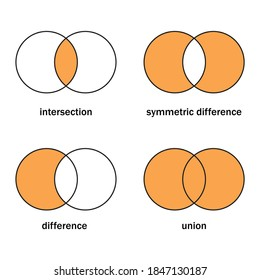
\includegraphics[width=0.5\textwidth]{figs/venn diagram.png}
\end{center}

\subsection{De-morgan's Law}
Let $A$ and $B$ be two sets then 
\begin{enumerate}
  \item $(A\cup B)^c = A^c \cap B^c$
  \item $(A\cap B)^c = A^c \cup B^c$
\end{enumerate}
\begin{myproof}
  Let $x \in (A \cup B)^c$ 
  \begin{align*}
    \implies & x \not \in A \cup B \\ 
    \implies & x \not \in A, x \not\in B \\
    \implies & x \in A^c , x \in B^c \\ 
    \implies & x \in A^c \cap B^c 
  \end{align*}
  Thus we can say that $(A\cup B)^c \subseteq A^c \cap B^c$\\
  Similarly Let $x \in A^c \cap B^c$.
  \begin{align*}
    \implies & x \in A^c , x \in B^c \\ 
    \implies & x \not \in A, x \not\in B \\
    \implies & x \not \in A \cup B \\ 
    \implies & x \in (A\cup B)^c
  \end{align*}
  Thus we can say that $A^c \cap B^c\subseteq(A\cup B)^c $\\
  This is possible iff $(A\cup B)^c = A^c \cap B^c$
\end{myproof}

\subsection{Partition of sets}
Let $S$ be a non-empty set. Then $S$ has the partition if it has a collection of subsets $A_i$ such that:
\begin{enumerate}
  \item $\forall a \in S, \exists $ unique $i$ such that $a \in A_i$
  \item $A_i \cup A_j = \phi, i \neq j$
\end{enumerate}
\begin{example}
  Consider the set $S = \{ 1,2, \dots, 9\}$\\ 
  \begin{enumerate}
    \item $[\{1,3,5\},\{2,6\},\{4,9\}]$
    \item $[\{1,3,5\},\{2,4,6,8\},\{7,9\}]$
  \end{enumerate}
  then $1$ is not a partition of $S$ as the element $7$ is missing. However $2$ is a partition of the set $S$.
\end{example}

\subsection{Relations}
A relation $R$ from set $A$ to set $B$ is subset of $A\times B$ where :
\[
  A\times B = \{(a,b) : a\in A, b\in B\}
\]
\[
  R \subseteq A \times B = \{(a,b) : a\in A, b\in B\}
\]

\begin{itemize}
  \item Domain $\rightarrow$ All the elements of set $A$
  \item Codomain $\rightarrow$ All the elements of set $B$
  \item Range $\rightarrow$ All the second elements of $R$
\end{itemize}
\begin{example}
  \begin{align*}
    R = & \{ (a,b) : b = 2a + 1, a \in [1,10] , b \in [1,10]\}\\
    A = & [1,10]\\
    R \subseteq & A \times A\\
    = & \{(1,3),(2,5),(3,7),(4,9)\}
  \end{align*}
  \begin{itemize}
    \item Domain = $\{1,2,3,4\}$
    \item Range = $\{3,5,7,9\}$
  \end{itemize}
\end{example}
\subsubsection{Composition of Relations}
Let $R$ be a relation from $A$ to $B$\\
Let $S$ be a relation from $B$ to $C$

then 
\[
  R \circ S = \{(a,c) : \exists b \in B \ s.t.\ (a,b) \in R, (b,c) \in S\}
\]
\begin{example}
  \begin{align*}
    \text{Let } & A = \{1,2,3,4\} \\
        & B = \{a,b,c,d\} \\
        & C = \{x,y,z\}\\
        & R = \{(1,a), (2,a), (3,a), (4,d)\}\\
        & S = \{(a,y), (b,x), (c,z)\}\\
    \implies & R \circ S = \{(1,y), (2,y), (3,z)\}
  \end{align*}
\end{example}
% TODO create matrix example for composition
\subsubsection{Equivalence Relations}
A relation $R$ from $A$ to $A$ is said to be equivalence if it satisfies the following conditions:
\begin{enumerate}
  \item Reflexivity
  \item Transivity
  \item Symmetricity
\end{enumerate}

\begin{definition}
  A relation is said to be reflexive iff:
  \[
    (a,a) \in R \ \forall a \in A
  \]
\end{definition}
\begin{definition}
  A relation is said to be Transitive iff:
  \[
    (a,b) \in R, (b,c) \in R \implies (a,c) \in R
  \]
\end{definition}
\begin{definition}
  A relation is said to be Symmetric iff:
  \[
    (a,b) \in R  \implies (b,a) \in R
  \]
\end{definition}
\begin{example}
  Consider the relation $R$ on $A = \{1,2,3,4\}$\\
  \begin{align*}
    &R_1 = \{(1,1), (1,2), (2,3), (1,3), (4,4)\}\\
    &R_2 = \{(1,1), (1,2), (2,1), (2,2), (3,3), (4,4)\}\\
    &R_3 = \{(1,3), (2,1)\}\\
    &R_4 = A \times A
  \end{align*}
  Then 
  \begin{itemize}
    \item $R_1$ is Transitive only
    \item $R_2$ is Equivalence
    \item $R_3$ is neither Symmetric, Reflexive or Transitive only
    \item $R_4$ is Equivalence
  \end{itemize}
\end{example}
\begin{definition}
  A relation on a set $A$ is said to be Anti-symmetric if and only if:
  \[
    (a,b) \in A, (b,a) \in A \implies a = b
  \]
\end{definition}
\subsection{Functions}
A relation from set $A$ to $B$ such that each element of $A$ has a unique mapping in $B$ then it is called a function and is denoted as 
\[
  f: A \rightarrow B
\]
All functions are relations but not vice-versa. 
\subsubsection{Domin, Range and Codomain}
for $f: A \rightarrow B$
\begin{itemize}
  \item Domain: $A$
  \item Codomain: $B$
  \item Range: $\{b \in B: \exists a \in A \text{ such that } f(a) = b\}$
\end{itemize}
Note:
\indent  Domain$(f) \subseteq A$\\
\indent  Range$(f) \subseteq B$\\
\subsubsection{One-one and Onto function}
Let $f:A\rightarrow B$ be a funciton then $f$ is called one-one if distinct elements of $A$ have different image.\\
Mathematically:
\[
  f(x_1) = f(x_2) \implies x_1 = x_2
\]

$f$ is said to be onto if each element of $B$ has a preimage in $A$.\\
Mathematically
\[
  \forall b \in B, \exists a \in A \text{ such that } f(a) = b
\]

\begin{definition}
  f is bijective iff it is both one-one and onto
\end{definition}

\subsubsection{Geometrical characterisation of one-one and onto functions}
\begin{centering}
  \begin{table}
    \begin{tabular}{c l}
      One-one & Each horizontal line cuts the graph at atmost one point\\
      Onto & Each horizontal line cuts the graph at one or more points\\
    \end{tabular}
  \end{table}
\end{centering}
\begin{example}
  Let $f: \mathbb{R} \to \mathbb{R}$ such that $f(x) = x^2$\\ 
  One-one: 
  \begin{align*}
    \text{Let }&f(x_1) = f(x_2) \\
    \implies & x_1^2 = x_2^2 \\
    \implies & x_1^2 - x_2^2 = 0 \\
    \implies & (x_1 - x_2)(x_1 + x_2) = 0 \\
    \implies & x_1 = x_2 \text{ or } x_1 = -x_2\\
  \end{align*}
  Onto:
  We have $f(x) = x^2 \geq 0$\\
  $\not \exists x < 0 \in \mathbb{R} \text{ such that } f(x) = x^2$
\end{example}
\subsection{Composition of Functions}
Let $f:A\to B$ and $g:B\to C$ be two functions then\\
$g\circ f: A\to C$ is called composition of $f$ and $g$.
\[
  g\circ f(x) = g(f(x))
\]
Result:\\
Let $ f:A\to B$ and $g:B\to C$ be two functions then
\begin{enumerate}
  \item $g\circ f$ is one-one if both $f$ and $g$ are one-one
  \item $g\circ f$ is onto if both $f$ and $g$ are onto
\end{enumerate}
\begin{myproof}
  \begin{enumerate}
    \item Let $(g\circ f)(x_1) = (g\circ f)(x_2)$
      \begin{align*}
        \implies & g(f(x_1)) = g(f(x_2)) \\ 
        \implies & f(x_1) = f(x_2) \text{ as g is one-one}\\ 
        \implies & x_1 = x_2 \text{ as f is one-one}\\
      \end{align*}
    \item $g\circ f: A \to C$ \\
      Let $z\in C$, we will show that $\exists x\in A$ such that $g\circ f(x) = z$\\
      Since $g$ is onto $\implies \exists y\in B$ such that $g(y) = z$\\
      Since $f$ is onto and $y\in B \implies \exists x \in A \text{ such that } f(x)=y$ 
  \end{enumerate}
\end{myproof}
\subsection{Induction}
Used to prove that a statement is true for all integers or natural numbers.
\[
  P(n) \text{ holds } \forall n
\]
\subsubsection{Principle of Mathematical Induction}
Let $P(n)$ be the given statement.
\begin{enumerate}
  \item \underline{Basic Step}: $P(1)$ is true
\item \underline{Induction Step}: $P(k) \implies P(k+1)$ is true
\end{enumerate}
This causes a domino effect and effectively proves that $P(n)$ is true $\forall n$
\begin{example}
  Using Induction, Prove that:
  \[
    1 + 2 + 3 + 4 + 5 + \dots + n = \frac{n(n+1)}{2}, n \in \mathbb{Z}^+
  \]
  \begin{enumerate}
    \item Base Case: \\ 
      \[
        1 = \frac{1(1+1)}{2} = 1
      \]
      \hfill Q.E.D.
    \item Induction Step:
      Let $P(k)$ is true, then we have to show that   $P(k+1)$ is true.
      \begin{align*}
        1+2+ \dots + k &= \frac{k(k+1)}{2} \\
        \implies 1+2+ \dots + k + (k+1) &= \frac{k(k+1)}{2} + (k+1) \\
        \implies 1+2+ \dots + k + (k+1) &= \frac{k(k+1)}{2} + \frac{2(k+1)}{2} \\
        \implies 1+2+ \dots + k + (k+1) &= \frac{(k+1)(k+2)}{2}
      \end{align*}
      \hfill Q.E.D.
  \end{enumerate}
\end{example}
\subsection{Recursion}
This is used when we cannot explicitly represent any object or mathematical term. so we use recursion.\\
\begin{definition}
  \underline{Recursive function}\\
  Let $\{a\}_n, n \in \mathbb{Z}^+_0$ such that $a_n\in \mathbb{Z} \forall n$ then:
  \begin{enumerate}
    \item Basic Step: $a_n$ is given at $n = 0$
    \item Recursive step: $a_n = f(a_{n-1},a_{n-2} \dots)$
  \end{enumerate}
\end{definition}
Well known examples of recursive expressions are: 
\begin{enumerate}
  \item Arithemetic progression
    \[
      a_n = a_{n-1} + d
    \]
  \item Geometric progression
    \[
      a_n = ra_{n-1}
    \]
  \item Factorial function
    \[
      f(n) = n \times f(n-1)
    \]
    \[
      f(0) = 1
    \]
  \item Fibonacci function
    \[
      f(n) = f(n-1) + f(n-2)
    \]
    \[
      f(0) = 0
    \]
    \[
      f(1) = 1
    \]
\end{enumerate}
\subsubsection{Linear recurrence relations with constant coefficients}
Let $a_n = \phi(a_{n-1},a_{n-2},\dots,a_{0},m)$\\ 
It can be written as:
\[
  a_n = c_1 a_{n-1} + c_2 a_{n-2} + \dots + c_{n-1} a_1 + c_n a_0 + f(m)
\]
If $f(m) = 0$ then the function is called homogeneous\\
If $f(m) \neq 0$ then the function is called non-homogeneous\\

\vspace{1cm}

\textbf{HOMOGENEOUS SOLUTION}\\
Note: $k$th order recurrence relation is one such that\[
  a_n = \phi(a_{n-1},a_{n-2},\dots,a_{n_k},m)
\]
or 
\[
  a_n = c_1a_{n-1} + c_2a_{n-2} + \dots + c_ka_{n-k} +  f(m)
\]
so a second order recurrence relation will look like:
\begin{equation}
  a_n = c_1a_{n-1} + c_2a_{n-2} + c_3
\end{equation}
Then characteristic equation of (1) is given by:
\[
  x^2 - c_1x - c_2 = 0, c_1,c_2 \in \mathbb{R}
\]
Come forth 3 cases: 
\begin{enumerate}
  \item When roots are real and distinct: \\
    \[
      x^2 - c_1x-c_2 = 0 \implies\begin{cases}
        x = r_1 \\ 
        x = r_2
      \end{cases}
      r_1 \neq r_2
    \]
    Then the solution of (1) is given by:
    \[
      a_n = p_1r_1^n + p_2 r_2^n
    \]
  \item Roots are real and equal:
    \[
      r_1 = r_2 = r
    \]
    Then the solution of (1) is given by:
    \[
      a_n = (p_1 + np_2) r^n
    \]
    \begin{example}
      Solve $a_n = 2a_{n_1} + 3a_{n-2}$
      \begin{align*}
        a_n - 2a_{n-1} - 3a_{n-2} &= 0\\
        \implies x^2 - 2x - 3 &= 0\\
        \implies (x-3)(x+1) = 0\\ 
        \implies x = -1, 3
      \end{align*}
      Solution: 
      \[
        a_n = p_1(-1)^n + p_2(3)^n
      \]
      Suppose: $a_0 = 1, a_1 = 2$
      \begin{align*}
        n = 0 &\implies a_0 = p_1(-1)^0 + p_2(3)^0\\
              &\implies 1 = p_1 + p_2\\
        n = 1 &\implies a_1 = p_1(-1)^1 + p_2(3)^1\\
              &\implies 2 = -p_1 + 3p_2\\
      \end{align*}
      From the above 2 equations we get:
      \begin{align*}
        p_1 = \frac{1}{4}\\
        p_2 = \frac{3}{4}
      \end{align*}
      \[
        \implies a_n = \frac{1}{4} (-1)^n + \frac{3}{4} (3)^n
      \]
    \end{example}
    \begin{example}
      Solve: $a_n = 6a_{n-1} - 9a_{n-2}$\\
      with $a_1 = 3, a_2 = 27$
      % TODO complete this example
    \end{example}
\end{enumerate}

\textbf{NON-HOMOGENEOUS SOLUTION}\\
We have
\begin{equation}
  a_n = c_1 a_{n-1} + c_2 a_{n-2} + \dots + c_k a_{n-k} + f(n)
\end{equation}
\\
where $f(n) \neq 0$\\ 
From (2) the associated homogeneous linear recurrence relation is
\begin{equation}
  a_n = c_1 a_{n-1} + \dots + c_k a_{n-k} 
\end{equation}
We can get the solution of (3), Let say ($a_n^c$)\\
Let $a_n^p$ is the particular solution of (2). Then the general solution of (2) can be written as 
\[
  a_n = a_n^c + a_n^p
\]

\begin{mytheorem}
  Suppose that $a_n$ satisfies the relation 
  \[
    a_n = c_1 a_{n-1} + c_2a_{n-2} + \dots + c_k a_{n-k} + f(n)
  \]
  where $c_i \in \mathbb{R} \forall i$ and 
  \[
    f(n) = (b_tn^t + b_{t-1}n^{t-1} + \dots + b_1n+b_0) s^n 
  \]
  where $b_i, s \in \mathbb{R} \forall i$

  Then the following cases.
  \begin{enumerate}
    \item If $s$ is not the root of the characteristic equation then the particular solution of (2) is of the type
      \[
        (p_tn^t + p_{t-1}n^{t-1} + \dots + p_1n + p_0 ) s^n
      \]
    \item if $s$ is root of the characteristic equation then the particular solution of (2) is of the type 
      \[
        n^m(p_tn^t + p_{t-1}n^{t-1} + \dots + p_1n + p_0 ) s^n
      \]
      where $m$ is the multiplicity of the root
  \end{enumerate}
\end{mytheorem}
\begin{example}
  Write the type of particular solution for the recurrence relation, $a_n = 6a_{n-1} -9a_{n-2} + f(n)$
  \begin{enumerate}
    \item $f(n) = 3^n$
    \item $f(n) = n3^n$
    \item $f(n) = n^2 2^n$
  \end{enumerate}
  \begin{solution}
    The associated homogeneous linear recurrence relation:
    \[
      a_n - 6 a_{n-1} + 9a_{n-2} = 0
    \]
    So characteristic equation :
    \[
      x^2  - 6x + 9 = 0
    \]
    \[
      \implies (x-3)^2 = 0
    \]
    \[
      \implies x = 3,3
    \]
    \begin{enumerate}
      \item $f(n) = 3^n$\\
        comparing to $f(n) = (b_tn^t + b_{t-1}n^{t-1} + \dots + b_1n+b_0) s^n$ we get\\
        so
        \[
          b_0 = 1, b_i = 0 \forall i > 0
        \]
        \\ 
        $s = 3$ is root of the characteristic equation with multiplicity 2\\
        So particular solution would be: 
        \[
          n^2 p_0 3^n
        \]
      \item $f(n) = n3^n$\\
        comparing to $f(n) = (b_tn^t + b_{t-1}n^{t-1} + \dots + b_1n+b_0) s^n$ we get\\
        so
        \[
          b_0 = 1, b_1 = 1, b_i = 0 \forall i > 1
        \]
        \\ 
        $s = 3$ is root of the characteristic equation with multiplicity 2\\
        So particular solution would be: 
        \[
          n^2 (p_1n + p_0) 3^n
        \]
      \item $f(n) = n^22^n$\\
        comparing to $f(n) = (b_tn^t + b_{t-1}n^{t-1} + \dots + b_1n+b_0) s^n$ we get\\
        so
        \[
          b_0 = 1, b_1 = 1, b_2 = 1, b_i = 0 \forall i > 1
        \]
        \\ 
        $s = 2$ is root of the characteristic equation with multiplicity 2\\
        So particular solution would be: 
        \[
          a_n^p = (p_2n^2+ p_1n + p_0) 2^n
        \]
        \[
          a_n^c = (c_1 + c_2n) 3^n
        \]
        From the above 2 equations ; 
        \begin{equation*}
          (p_2 n^2 c p_1n + p_0) 2^n = 6(p_2(n-1)^2 + p_2(n-1) +p_0) 2^{n-1} - 9 (p_2(n-2)^2 + p_1(n2)+p_0)2^{n-2} + n^22^n 
        \end{equation*}
    \end{enumerate}
  \end{solution}
  \begin{example}
    Solve:
    \[
      a_n = 6a_{n-1}- 9 a_{n-2} + n^22^n , a_0 = 1, a_1 = 2
    \]
    \begin{solution}
      The associated homogeneous linear recurrence relation is $a_n = 6a_{n-1} - 9a_{n-2}$
      So the characteristic equation is
      \begin{align*}
        x^2 - 6x + 9 &= 0 \\         
        \implies x &= 3,3
      \end{align*}
      So 
      \[
        a_n^c = (c_1 + c_2n) 3^n
      \]
      for particular solution: 
      \[
        a_n^p = (b_2 n^2 + b_1 n + b_0) 2^n
      \]
      so the general solution :
      \[
        a_n = (c_1 + c_2n)3^n + (b_2 n^2 + b_1 n + b_0) 2^n
      \]
      putting the values of $a_0$ and $a_1$ we get 
      \begin{align*}
        1 &= c_1 3^0 + b_0 2^n \\ 
        \implies 1 &= c_1 + b_0\\ \\ 
        2 &= (c_1 + c_2) 3 + (b_2+ b_1 + b_0)2\\
        \implies 2 &= 3c_1 + 3c_2 + 2b_2 + 2b_1 + 2b_0
      \end{align*}
      Comparing the coefficients of $2^n$ and $3^n$ in both sides: 
      \begin{align*}
        b_0 + b_1 + b_2 &= 1\\ 
        c_1 + c_2 &= 0\\ 
        c_1 &= 1\\ 
        b_0 &= 0\\ 
        c_2 &= -c_1 = -1
      \end{align*}
    \end{solution}
  \end{example}
\end{example}

\section{Logic and Proof Techniques}

\begin{definition}
  Proposition(statement): is a declarative sentence that is either true or false but not both.
\end{definition}

\begin{example}
  \begin{enumerate}
    \item Ice floats on water. 
    \item $2-x = 3$
  \end{enumerate}
\end{example}
\subsection{Proof Techniques}
\begin{definition}
  \textbf{Conjecture:} Any statement given is a conjecture.\\
  \textbf{Theorem:} A statement which is to be proved true.\\
  \[
    Conjecture + proof \rightarrow Theorem
  \]
  \textbf{Proof:} The technique by which we check whether the given statement is true or not\\
\end{definition}

There are the following proof techniques:

\begin{enumerate}
  \item Direct Proof
  \item Proof by Contrapositive
  \item Proof by Contradiction
  \item Proof by Counterexample
  \item Proof by Cases
\end{enumerate}

\subsubsection{Direct Proof}
If we are given $p \to q$, then take $p$ and by implications of $p$, we arrive at $q$.\\
\begin{example}
  If $n$ is even then prove that $n^2$ is even.\\

  Given: $n$ is even.\\
  To prove: $n^2$ is even\\
  Proof: let us say that \\
  \begin{align*}
    n &= 2k, k \in \mathbb{Z}\\
    \implies n^2 &= 4k^2\\
    \implies n^2 &= 2(2k^2)\\
  \end{align*}
\end{example}
\begin{example}
  For all integers $a$,$b$ and $c$ if $a|b$, and $b|c$ prove that $a|c$

% TODO complete this
\end{example}

\subsubsection{Proof by Contrapositive}
Suppose we have to prove that $p \implies q$, then it is equivalent to proving $\neg q \implies \neg p$

\begin{example}
  For all integers $a$ and $b$ if $a+b$ in odd then either $a$ is odd or $b$ is odd

  $p: a+b$ is odd\\
  $q: a$ is odd or $b$ is odd\\

  $\neg p: a+b$ is even\\
  $\neg q: a$ is even and $b$ is even\\
  
  since $p \implies q \equiv \neg q \implies \neg p$\\
  We have $a$ is even and $b$ is even \\ 
  \[
    a = 2m, b = 2n, m,n \in \mathbb{Z}
  \]
  \begin{align*}
    \implies a+b &= 2m +2n\\
                &= 2(m+n)\\
                &= 2k , k \in \mathbb{Z}
  \end{align*}
\end{example}

\begin{example}
  For every prime number $r$, if $r\neq 2$ then $r$ is odd
\end{example}

\subsubsection{Proof by Contradiction}
We have co prove $p \implies q$\\ 
Then it is equivalent to $\neg p \implies \neg q$\\

for that we take $p$ is not true and then by implications, we arrive at some Contradiction.

\begin{example}
  $\sqrt 2$ is irrational. \\ 

  suppose $\sqrt 2$ is a rational number.\\ 
  Then we can represent it in form of $\frac{p}{q}$ such that $p$ and $q$ are coprimes\\

  \begin{align*}
    \implies &\sqrt 2 = \frac{p}{q}\\
    \implies & 2 = \frac{p^2}{q^2}\\
    \implies & 2 q^2 = {p^2}\\
  \end{align*}

  hence $p$ is an even number.
  therefore we can write $p$ as 
  \[
    p = 2k 
  \]
  \[
    p^2 = 4k^2
  \]
  \[
    2q^2 = 4k^2
  \]
  \[
    q^2 = 2k^2
  \]

  thus $q$ is also an even number.\\ this is a contradiction to the fact that $p$ and $q$ are coprime.
\end{example}


\section{Lattice}

\subsection{Complement of an element}
Let $L$ be a Lattice then an element $b \in L$ is said to be complement of $a\in L$ if 
\[
  a * b = 0
\]
\[
  a \oplus b = 1
\]

An element may have no complement, unique complement or more than one complements

\begin{mytheorem}
  The following conditions always hold true:
  \[
    0' = 1
  \]
  \[
    1' = 0
  \]
  and these complements are unique
\end{mytheorem}

\begin{definition}
  A lattice $L$ is complemented if each element has atleast one complement. 
\end{definition}

\begin{definition}
  A Lattice is said to be distributive if 
  \[
    a * (b \oplus c) = (a * b) \oplus (a * c)
  \]
  \[
    a \oplus (b * c) = (a \oplus b) * (a \oplus c)
  \]
  This is true if each element has atmost one complement.
\end{definition}

\subsection{Boolean Algebra}
\begin{definition}
  A Lattice is Boolean if it is both complementary and distributive i.e. each element of  lattice has exactly one complement. 
  Alternatively, A Lattice is Boolean if it is isomorphic to a $D_n$(divisors of n).
\end{definition}

\begin{example}
  %TODO insert example, like that diamond thingy and exam example for not boolean 
\end{example}

\begin{mytheorem}
  \noindent Here are some results to keep in mind.
  \begin{enumerate}
    \item If a lattice does not contain $2^n$ elements then it cannot be a boolean lattice.
    \item if $\lvert L\rvert = 2^n$ Then it may or may not be boolean.
    \item if $n = p_1 \times p_2 \times \dots p_k$ where each $p_i$ is a distinct prime then $L$ will be a boolean algebra.
    \item Let $n \in \mathbb{Z}$ and $p^k | n$ for some $k > 1$ then $D_n$ is not a boolean algebra
  \end{enumerate}
\end{mytheorem}

\subsection{Logic Gates and Circuits}

Basic type of logic gates:
\begin{enumerate}
  \item OR Gate
  \item AND Gate
  \item NOT Gate
\end{enumerate}

\subsubsection{OR Gate}

\[
  Y = A * B \equiv A + B 
\]

$Y$ will be 0 if and only if $A$ and $B$ both are zero.

\subsubsection{AND Gate}

\[
  Y = A \oplus B \equiv A \cdot B
\]

$Y$ will be 1 if and only if $A$ and $B$ both are 1.

\subsubsection{NOT Gate}

\[
  Y = A' = \overline{A}
\]

$Y$ will just be the opposite of $A$.

\subsubsection{Logic Circuit}
\begin{definition}
  Any combination of logic gates to get the desired output is called logic circuit.

  Note that logic circuit follows the rules of boolean algebra.
\end{definition}

\subsubsection{NAND and NOR Gate}

NAND Gate is the combination of AND and NOT Gate. \\ 
NOR Gate is the combination of OR and NOT Gate.

% TODO: Create the Truth Tables of these. Also read about k-maps.


\section{GROUP THEORY yeah imma kms}
  
\subsection{Binary Operations}

\begin{definition}
  Let $A$ be a set then any operation $*$ on $A$ is binary operation if $\forall a, b \in A, a*b \in A$. 
  For example, $(\mathbb{Z},+)$ is a group, but $(\mathbb{Z},/)$ is not.
\end{definition}

\subsection{Group}

\begin{definition}
  Let $G$ be a nonempty set with a defined binary operation $*$ then $G$ is called group if it satisfies a certian condition. 
  \begin{enumerate}
    \item Closure: $a*b \in G \forall a,b \in G$.
    \item Associativity: $(a*b)*c = a*(b*c)$.
    \item Existence of Identity: $\exists e \in G, a*e = a \forall a \in G$.
    \item Existence of Inverse: $\forall a \in G\ \exists\ b \in G$ such that $a*b = e$
  \end{enumerate}
\end{definition}

\begin{example}
  $(\mathbb{Z},+)(\mathbb{Q},+)(\mathbb{R},+)$ are groups\\
  $(\mathbb{Z},-)$ is not a group because $-$ is not associative\\
  $(\mathbb{N},+)$ is not a group because there does not exist an identity in $\mathbb{N}$\\ 
  $(\mathbb{Z},\cdot)$ is not a group because there is no inverse for $a \in \mathbb{N}$\\
  $(\mathbb{R},\cdot)$ is not a group because there is no inverse for $0 \in \mathbb{R}$\\
  $(\mathbb{R}\setminus \{0\},\cdot)$ is a group. 
\end{example}

\begin{example}
  let $X = \mathbb{M}(\mathbb{R})_{2\times 2}$, then $G = (X, +)$ is a group.\\ 
  However $G' = (X, \cdot)$ is not a group as there may or may not exist an inverse for a real matrix.
\end{example}

\subsection{Abelian Group}
Let $G$ be a group with binary operation * then $G$ is abelian if 
\[
  a*b = b*a \forall a,b \in G
\]

\begin{example}
  $(\mathbb{Z}, +)$ is a group where $a + b = b + a \forall a,b \in \mathbb{Z}$ \\
  Thus $(\mathbb{Z}, +)$ is an abelian group.
\end{example}

\begin{example}
  $GL(2, \mathbb{R}) = $ group of non singular matrices of order 2 with real entities\\ 
  note that it is not necessary that the product of two matrices be commutative.
\end{example}

\begin{example}
  $SL(2, \mathbb{R}) = $ group of matrices of order 2 with real entities and determinant 1\\ 
  note that it is not necessary that the product of two matrices be commutative.
\end{example}

\subsection{Unitary group}

\begin{definition}
\[
  U(n) = \{a:a\in\mathbb{Z}, gcd(a,n) = 1, a < n\}
\]
\end{definition}

\begin{example}
\[
  U(10) = \{1,3,7,9\}
\]

Note that $(U(10), \odot_n)$\\
$\odot_n$ is multiplication moduolo
\end{example}

Note: 
\[
  a \oplus_n b = a + b \pmod n
\]
\[
  a \odot_n b = a \cdot b \pmod n
\]

\subsubsection{Cayley Table}
It is a visual table representation of a group. we just multiply the group with itself to check for inverses\\

\begin{example}
  \[
    \mathbb{Z}_n = \{0,1, \dots, n-1\}
  \]
  then $(\mathbb{Z}_n,\oplus_n)$ is a group with identity 0.\\
  and $<\mathbb{Z}_n, \oplus_n>$ is an abelian group.
\end{example}


\subsection{Properties of a group}
\begin{enumerate}
  \item Uniqueness of identity\\ 
    The identity of the group must be unique. To prove take two distinct identities and show that they are equal.
  \item Cancellation Laws:- \\
    Let $G$ be a group and $a,b,c \in G$. Then 
    \begin{enumerate}
      \item $ab = ac \implies b = c$ (left cancellation law) 
      \item $ab = cb \implies a = c$ (right cancellation law)
    \end{enumerate}
  \item Uniqueness of inverse
  \item Let $G$ be a group then $(ab)^{-1} = b^{-1}a^{-1}$
  \item Let $G$ be an abelian group then $(ab)^{-1} = b^{-1}a^{-1} = a^{-1}b^{-1}$
\end{enumerate}

\begin{myproof}
  \begin{enumerate}
    \item 
    \item 
      \begin{enumerate}
        \item To show: $ab = ac \implies b = c$ \\
          Proof: 
          \begin{align*}
            ab &= ac \\ 
               &\text{ since $G$ is a group $\exists a^{-1} \in G$. So premultiply by $a^{-1}$}\\
            a^{-1}ab &= a^{-1}ac \\ 
            eb &= ec \\ 
            b &= c \\ 
          \end{align*}
      \end{enumerate}
    \item Let $G$ be a group and $a \in G$. 
      Let $b, c$ be the inverses of $a$. 
      since $b$ is inverse of $a$:
      \[
        ab = ba = e 
      \]
      similarly
      \[
        ac = ca = e 
      \]
      From the two above statements we can infer that: 
      \[
        ab = ac = e
      \]
      From the left cancellation law
      \[
        b = c
      \]
  \end{enumerate}
\end{myproof}

\subsection{Subgroups}
\begin{definition}
  The order of a group is the number of elements in a group.\\
  \begin{example}
    \[
      G = U(10) = \{1,3,7,9\}
    \]
    \[
      O(G) = 4
    \]
  \end{example}
\end{definition}

\begin{definition}
  \textbf{The order of an element in a group}\\
  Let $G$ be a group and $a \in G$ then oredr of $a$ is defined as:
  \[
    O(a) = \{n: a^n = e, a\in G\} (\cdot)
  \]
  \[
    O(a) = \{n: na = e, a\in G\} (+)
  \]
  then $n$ is called order of $a$
\end{definition}

\begin{definition}
  Let $H$ be subset of $G$ then $H$ is called subgroup of $G$ if $H$ itself is group under the same operation as that of $G$. \\
  Notation: $H \leq G$
\end{definition}

\begin{example}
  $(\mathbb{Z}, +) \leq (\mathbb{R}, +)$ 
\end{example}

\begin{example}
  $(\mathbb{Z}_{10}, \oplus_{10} \not\leq (\mathbb{R}, +)$ as the operation is not the same
\end{example}

\subsubsection{One step subgroup test}
Let $H$ be subset of the group $G$. Then $H$ is ssubgroup of $G$ if 
\[
  ab^{-1} \in H \forall a,b \in H (\text{wrt multiplication})
\]
\[
  a-b \in H \forall a,b \in H (\text{wrt addition})
\]

\begin{example}
  Let $G$ be a Abelian group with identity $e$ and $H = \{x \in G: x^2 = e\}$ then check for $H \leq G$

  by one step test: 
  \[
    ab^{-1} \in H \forall a,b \in H (\text{wrt multiplication})
  \]

  since $a,b \in H, a^2 = e, b^2 = e$

  so $(ab^{-1})^2 = ab^{-1}ab^{-1} = aab^{-1}b^{-1} = a^2 b^{-2} = e e^{-1} = e$\\
  Therefore $H \leq G$
  $\hfill \blacksquare$
\end{example}

\subsubsection{Two step subgroup test}
Let $G$ be a group and $H \subseteq G$ then iff: 
\begin{enumerate}
  \item $ab \in H \forall a, b \in H$
  \item $a \in H \forall a \in H$
\end{enumerate}

\begin{example}
  Let $G = GL(2,\mathbb{Z})$ with addition. \\ 
  Let $H = \Big\{ \begin{pmatrix} a & b \\ c & d \end{pmatrix} : a + b + c + d = 0 \Big\}$
\end{example}

\begin{example}
  $G = GL(2,\mathbb{R})$\\
  $H = \Big \{ \begin{pmatrix}
      a & 0 \\ 
      0 & b 
  \end{pmatrix} : a,b \in \mathbb{Z}\setminus \{0\} \Big\}$

  Then $H$ will not be a subgroup because there may or may not exist an inverse of $a \in H$ in $H$
\end{example}

\subsection{Cyclic groups}
a group $G$ is called cyclic if $G = <a>$ where 
\[
  <a> = \{a^n : n \in \mathbb{Z} \} \text{ With respect to multiplication}
\]
\[
  <a> = \{na : n \in \mathbb{Z} \} \text{ With respect to addtion}
\]

\begin{example}
  $U(10) = \{1,3,7,9\}$ under multiplication $\odot_{10}$
  \begin{align*}
    3^1 = 3\\
    3^2 = 9\\
    3^3 = 7\\
    3^4 = 1\\
    3^5 = 3\\
  \end{align*}
  So $U(10)$ is cyclic
\end{example}

Note: in $\mathbb{Z}_n$, the generators are the numbers which are coprime to $n$. so $\mathbb{Z}_{10}$ has 1,3,7,9 as it's generators under addition modulo $n$

\subsubsection{Euler's phi (totient) function}

\[
  \phi(1) = 1
\]

for $n > 1$  

\[
  \phi(n) = \begin{cases}
    n-1, &n \text{ is prime}\\
    p^m - p^{m-1}, &n = p^m\\
    (p-1)(q-1), &n = pq\\
  \end{cases}
\]

\vspace{0.5in}

Note that $\mathbb{Z}$ has only $1$ and $-1$ as it's generators. It is also the only infinite cyclic group

\subsection{Subgroups of $\mathbb{Z}_n$}
For any divisor $k$ of $n$, the set $\langle \frac{n}{k} \rangle$ is a unique subgroup of order $k$ and thees are the only subgroup of $\mathbb{Z}_n$.

\begin{example}
  Let us take $\mathbb{Z}_{30}$

  \begin{align*}
    \langle \frac{30}{1} \rangle = \langle 30 \rangle &= \{ 0 \}\\
    \langle \frac{30}{2} \rangle = \langle 15 \rangle &= \{ 0, 15\}\\
    \langle \frac{30}{3} \rangle = \langle 10 \rangle &= \{ 0, 10, 20 \}\\
    \langle \frac{30}{5} \rangle = \langle 6\rangle &= \{ 0, 6, 12, 18, 24 \}\\
    \langle \frac{30}{6} \rangle = \langle 5\rangle &= \{ 0, 5, 10, 15, 20, 25\}\\
    \langle \frac{30}{10} \rangle = \langle 3 \rangle &= \{ 0, 3, 6, 9, 12, 15, 18, 21, 24, 27\}\\
    \langle \frac{30}{15} \rangle = \langle 2 \rangle &= \{ 0, 2, 4, 6, 8, 10, 12, \dots, 28\}\\
    \langle \frac{30}{30} \rangle = \langle 1 \rangle &= \{ 0, 1, 2, 3 ,4 , 5, 6 , \dots, 29\}\\
  \end{align*}
\end{example}

\subsection{Center of a group}
\[
  Z(G) = \{ x \in G ; xa = ax \forall a \in G \}
\]

in leyman terms, collection of all elements which commute with each other 

Note: if $G$ is abelian then $Z(G) = G$

\begin{example}
  if $G = GL(2,\mathbb{R}) = \left\{ \begin{pmatrix}
      a & b \\ c & d
  \end{pmatrix}: a,b,c,d \in \mathbb{R}\right\}$\\
  $Z(G) = \left\{ \begin{pmatrix}
      e & 0 \\ 0 & e 
  \end{pmatrix} : e \in \mathbb{R}\right\}$
\end{example}


\begin{fbox}
  {Note: $Z(G) \leq G$}
\end{fbox}

\subsection{Centralizer of an element}
for an element $a \in G$
\[
  C(a) = \left\{ x \in G : xa = ax \right\}
\]

Note: if $G$ is abelian then $C(a) = G$

\begin{example}
  \[
    G = GL(2,\mathbb{R})
  \]
  find $C\left( \begin{bmatrix}
      1& 1 \\ 1& 0
  \end{bmatrix}\right)$
   

  \noindent Suppose $\begin{pmatrix}
    a & b \\ c & d
  \end{pmatrix} \in G$

  \[
    \begin{pmatrix}
      a& b \\ c& b
    \end{pmatrix} \begin{pmatrix}
      1& 1\\ 1& 0
    \end{pmatrix} = \begin{pmatrix}
      1& 1\\ 1& 0
    \end{pmatrix} \begin{pmatrix}
      a& b \\ c& b
    \end{pmatrix}
  \]

  \[
    \begin{pmatrix}
      a+b & a \\ c+d & c
    \end{pmatrix} = \begin{pmatrix}
      a+c & b+d \\ a & b
    \end{pmatrix}
  \]
\end{example}

\subsection{Partition of numbers}
Let $n$ be a pasitive integer then teh ways in which the number can be written form partition of $n$.

\begin{example}
  \begin{align*}
    n = 1&, 1\\
    n = 2&, 2\\ 
         &, 1+1\\ 
    n = 3&, 3\\ 
         &, 2+1\\ 
         &, 1+1+1\\ 
    n = 4&, 4\\ 
         &, 3+1\\ 
         &, 2+2\\ 
         &, 2+1+1\\ 
         &, 1+1+1+1
  \end{align*}
\end{example}

Formula: \[
  P(n+1) = \sum_{r=0}^n {n \choose r} P(r) 
\]
given $P(0) = 1$

So 
\begin{align*}
  P(4) &= P(3+1)\\ 
       &= \sum_{r=0}^3 {3 \choose r} P(r)\\ 
       &= {3 \choose 0} P(0) + {3 \choose 1} P(1) + {3 \choose 2} P(2) + {3 \choose 3} P(3) \\
       &= 1 + 3\times 1 + 3\times 2 + 1\times 3
       &= 13
\end{align*}

\subsection{Order of elements in $S_n$}
Take $n$ and make the partitions of $n$.

\begin{example}
  \begin{align*}
    S_4 && 4 &\rightarrow LCM = 4\\
        && 1 + 3 &\rightarrow LCM = 3\\
        && 2 + 2 &\rightarrow LCM = 2\\
        && 1 + 1 + 2 &\rightarrow LCM = 1\\
        && 1 + 1 + 1 + 1 &\rightarrow LCM = 1
  \end{align*}
  It means that $S_4$ has elements of order 1, 2, 3, 4.\\
\end{example}

\noindent To find the number of elements of order $m$ in $S_n$. \\
Let $n = p_1 + p_2 + \dots$\\

\[
  \frac{n!}{p_1^{m_1} \cdot m_1! \times p_2^{m_2} \cdot m_2!}
\]
\end{document}
